\section{Abstract}\label{sec:abstract}

Noise pollution affects one in seven people in Switzerland, 
primarily caused by road traffic, railways, and air traffic, along with secondary sources such as construction sites and nightclubs. 
To address this issue, affected individuals must provide evidence, typically through audio recordings.
This project aims to create a free, open-source, and platform-independent application, which helps individuals in documenting noise pollution. \\
\\
The application processes *.wav files, filters the data by a given threshold and
generates a PDF with an according plot which can be used as evidence.
For a meaningful interpretation of a *.wav file, the user must provide a minimal and maximal dB(A) provided by an external tool,
such as smartphone apps like DecibelX. \\

\begin{table}[H]
    \centering
    \begin{tabularx}{\textwidth}{l X}
        \toprule
        License           & \textbf{\href{https://www.gnu.org/licenses/gpl-3.0.en.html}{GPL-3.0 licence (FLOSS)}} \\
        \midrule
        Application       & \textbf{\href{https://decibel-threshold-event-displayer.github.io/\#/}{dB threshold event displayer}} \\
        \midrule
        About Page        & \textbf{\href{https://decibel-threshold-event-displayer.github.io/\#/about}{About Decibel Threshold Event Displayer}} \\
        \midrule
        Repository        & \textbf{\href{https://github.com/decibel-threshold-event-displayer/decibel-threshold-event-displayer.github.io}{GitHub}} \\
        \bottomrule
    \end{tabularx}
    \label{tab:abstract-infos}
\end{table}

~\\

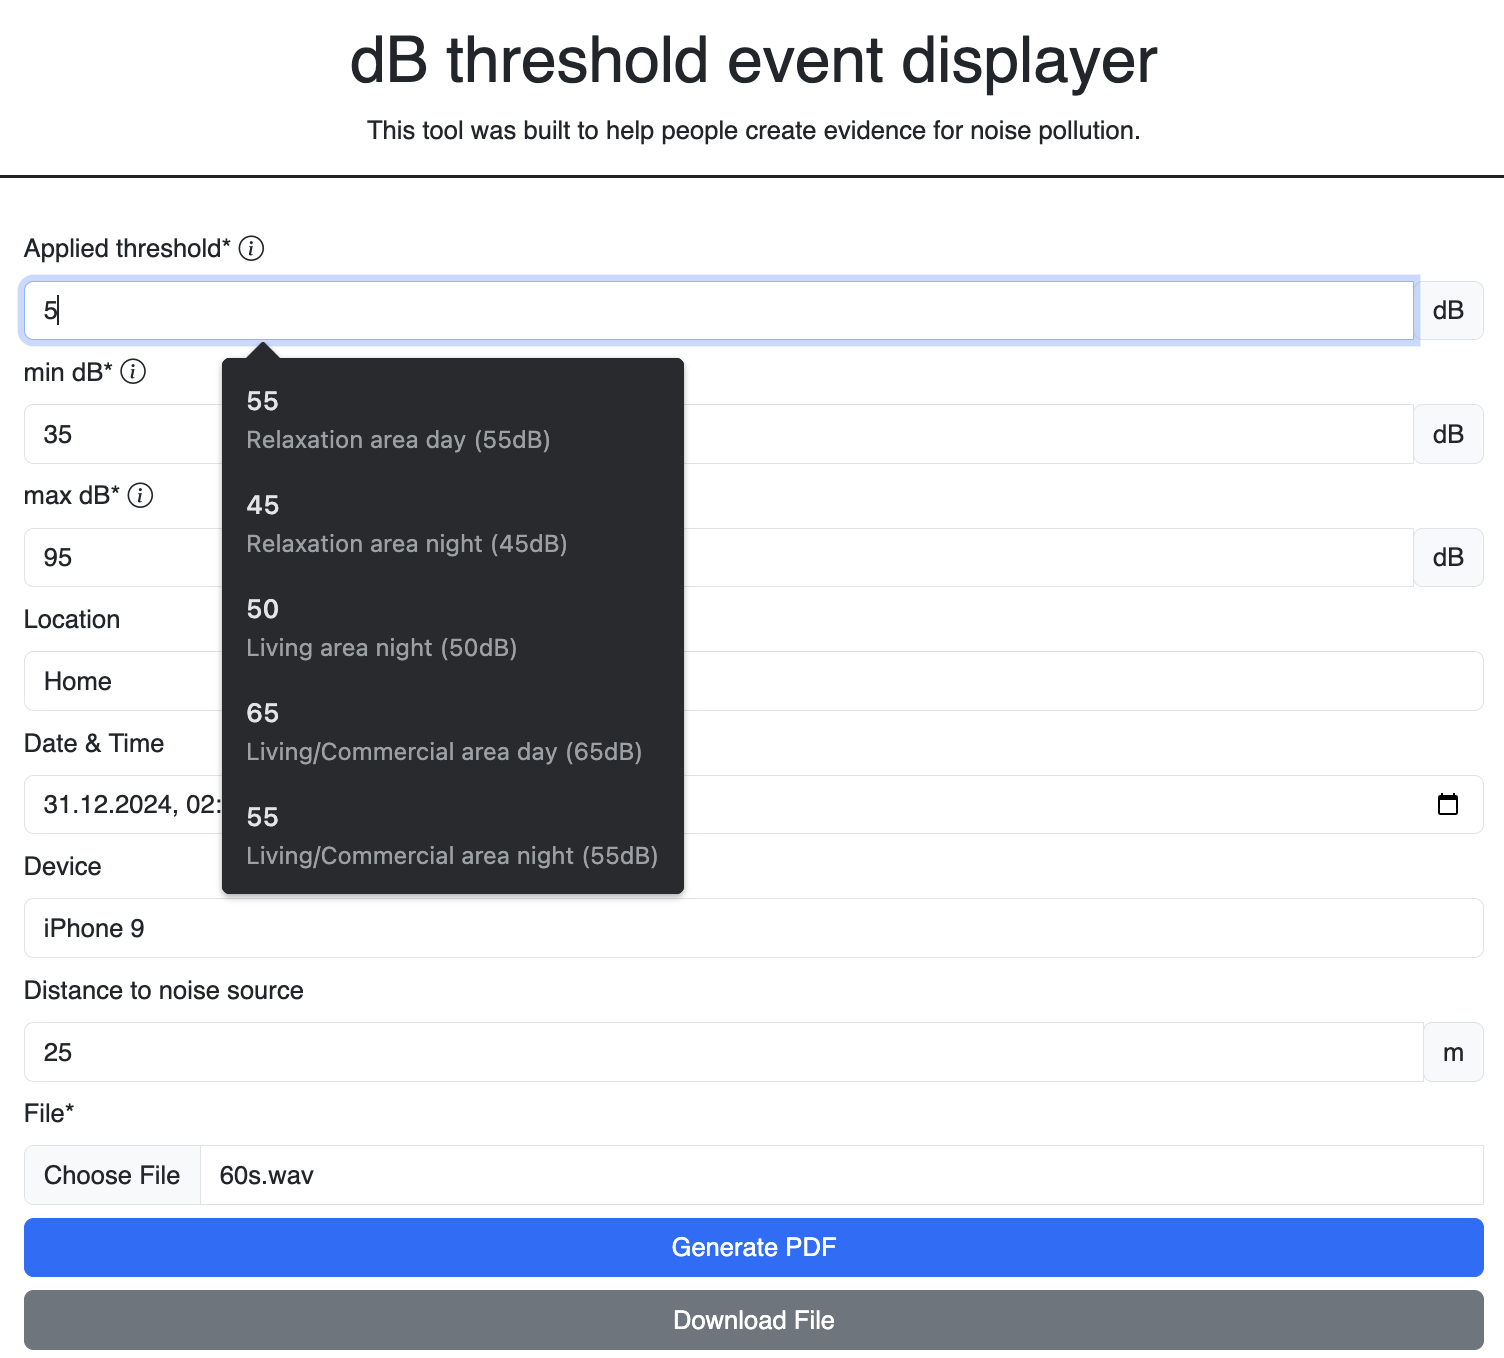
\includegraphics[width=0.475\textwidth]{../assets/abstract_application_screenshot.png}
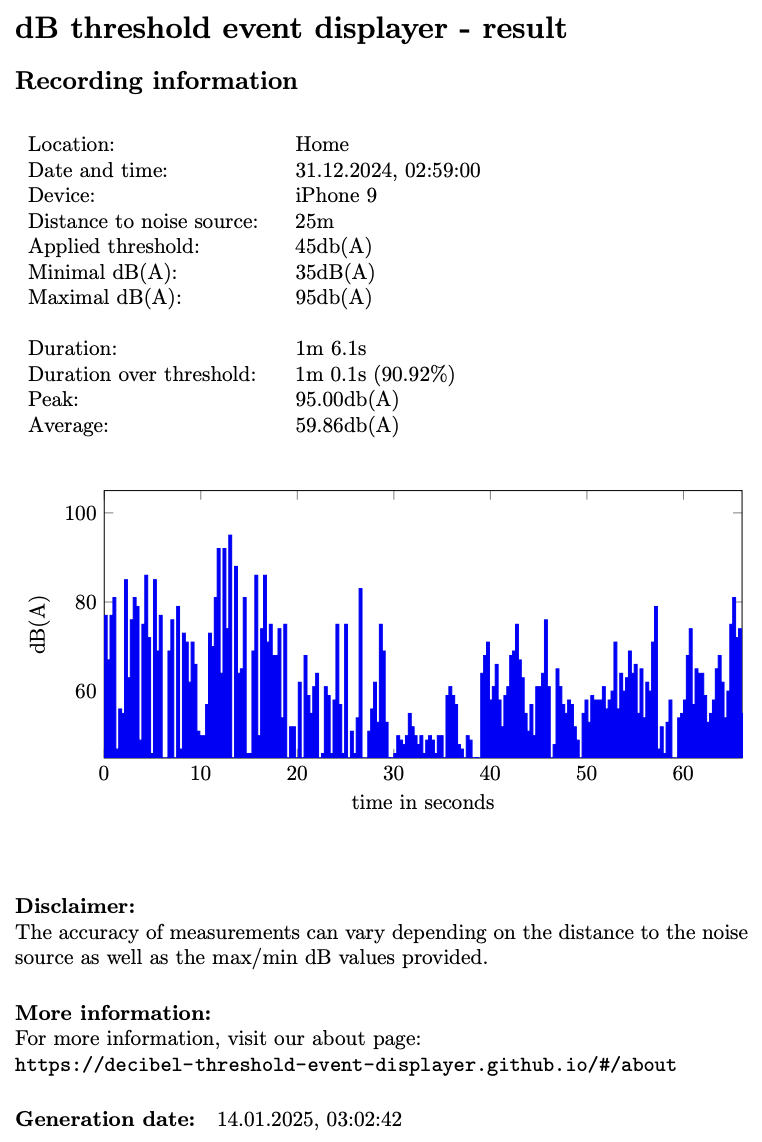
\includegraphics[width=0.475\textwidth]{../assets/abstract_report_screenshot.png}

\pagebreak
